%% This is file `prletters-template.tex',
%% 
%% Copyright 2013 Elsevier Ltd
%% 
%% This file is part of the 'Elsarticle Bundle'.
%% ---------------------------------------------
%% 
%% It may be distributed under the conditions of the LaTeX Project Public
%% License, either version 1.2 of this license or (at your option) any
%% later version.  The latest version of this license is in
%%    http://www.latex-project.org/lppl.txt
%% and version 1.2 or later is part of all distributions of LaTeX
%% version 1999/12/01 or later.
%% 
%% The list of all files belonging to the 'Elsarticle Bundle' is
%% given in the file `manifest.txt'.
%% 
%% Template article for Elsevier's document class `elsarticle'
%% with harvard style bibliographic references
%%
%% $Id: prletters-template-with-authorship.tex 69 2013-07-15 10:15:25Z rishi $
%%
%% This template has no review option
%% 
%% Use the options `twocolumn,final' to obtain the final layout
\documentclass[times,twocolumn,final,authoryear]{elsarticle}

%% Stylefile to load PR Letters template
\usepackage{prletters}
\usepackage{framed,multirow}
\usepackage[cjk]{kotex}
%% The amssymb package provides various useful mathematical symbols
\usepackage{amssymb}
\usepackage{latexsym}
\usepackage{multirow}

% Following three lines are needed for this document.
% If you are not loading colors or url, then these are
% not required.
\usepackage{url}
\usepackage{xcolor}
\definecolor{newcolor}{rgb}{.8,.349,.1}



\journal{Pattern Recognition Letters}

\begin{document}

\thispagestyle{empty}
                                                             
\begin{table*}[!th]

\begin{minipage}{.9\textwidth}
\baselineskip12pt
\ifpreprint
  \vspace*{1pc}
\else
  \vspace*{-6pc}
\fi

\noindent {\LARGE\itshape Pattern Recognition Letters}
\vskip6pt

\noindent {\Large\bfseries Authorship Confirmation}

\vskip1pc


{\bf Please save a copy of this file, complete and upload as the 
``Confirmation of Authorship'' file.}

\vskip1pc

As corresponding author 
I, \underline{ Rhee Man Kil\hphantom{\hspace*{5cm}}},
hereby confirm on behalf of all authors that:

\vskip1pc

\begin{enumerate}
\itemsep=3pt
\item This manuscript, or a large part of it, \underline {has not been
published,  was not, and is not being submitted to} any other journal. 

\item If \underline {presented} at or \underline {submitted} to or
\underline  {published }at a conference(s), the conference(s) is (are)
identified and  substantial \underline {justification for
re-publication} is presented  below. A \underline {copy of
conference paper(s) }is(are) uploaded with the  manuscript.

\item If the manuscript appears as a preprint anywhere on the web, e.g.
arXiv,  etc., it is identified below. The \underline {preprint should
include a  statement that the paper is under consideration at Pattern
Recognition  Letters}.

\item All text and graphics, except for those marked with sources, are
\underline  {original works} of the authors, and all necessary
permissions for  publication were secured prior to submission of the
manuscript.

\item All authors each made a significant contribution to the research
reported  and have \underline {read} and \underline {approved} the
submitted  manuscript. 
\end{enumerate}

Signature\underline{ Rhee Man Kil\hphantom{\hspace*{5cm}}} Date\underline{ March 11, 2016\hphantom{\hspace*{1.7cm}}} 
\vskip1pc

\rule{\textwidth}{2pt}
\vskip1pc

{\bf List any pre-prints:} none
\vskip5pc


\rule{\textwidth}{2pt}
\vskip1pc

{\bf Relevant Conference publication(s) (submitted, accepted, or
published):} none
\vskip5pc



{\bf Justification for re-publication:} not available

\end{minipage}
\end{table*}

\clearpage
\thispagestyle{empty}
\ifpreprint
  \vspace*{-1pc}
\fi

\begin{table*}[!th]
\ifpreprint\else\vspace*{-5pc}\fi

\section*{Graphical Abstract (Optional)}
To create your abstract, please type over the instructions in the
template box below.  Fonts or abstract dimensions should not be changed
or altered. 

\vskip1pc
\fbox{
\begin{tabular}{p{.4\textwidth}p{.5\textwidth}}
\bf Type the title of your article here  \\
Author's names here \\[1pc]
\includegraphics[width=.3\textwidth]{top-elslogo-fm1.pdf}
& 
This is the dummy text for graphical abstract.
This is the dummy text for graphical abstract.
This is the dummy text for graphical abstract.
This is the dummy text for graphical abstract.
This is the dummy text for graphical abstract.
This is the dummy text for graphical abstract.
This is the dummy text for graphical abstract.
This is the dummy text for graphical abstract.
This is the dummy text for graphical abstract.
This is the dummy text for graphical abstract.
This is the dummy text for graphical abstract.
This is the dummy text for graphical abstract.
This is the dummy text for graphical abstract.
This is the dummy text for graphical abstract.
This is the dummy text for graphical abstract.
This is the dummy text for graphical abstract.
This is the dummy text for graphical abstract.
This is the dummy text for graphical abstract.
This is the dummy text for graphical abstract.
This is the dummy text for graphical abstract.
This is the dummy text for graphical abstract.
This is the dummy text for graphical abstract.
This is the dummy text for graphical abstract.
This is the dummy text for graphical abstract.
%}\\
\end{tabular}
}

\end{table*}

\clearpage
\thispagestyle{empty}

\ifpreprint
  \vspace*{-1pc}
\else
%  \vspace*{-6pc}
\fi

\begin{table*}[!t]
\ifpreprint\else\vspace*{-15pc}\fi

\section*{Research Highlights (Required)}

To create your highlights, please type the highlights against each
\verb+\item+ command. 

\vskip1pc

\fboxsep=6pt
\fbox{
\begin{minipage}{.95\textwidth}
It should be short collection of bullet points that convey the core
findings of the article. It should  include 3 to 5 bullet points
(maximum 85 characters, including spaces, per bullet point.)  
\vskip1pc
\begin{itemize}

 \item Analyzing ECG signal data to check the condition of heat health

 \item The R-R intervals are analyzed by Gamma distribution parameters.

 \item Calculating the $p$-values for testing the heart condition using class probability output networks

 \item High accuracy and high recall for the abnormal heart condition

 \item Easy application to handheld or wearing devices with heart rate sensors

\end{itemize}
\vskip1pc
\end{minipage}
}

\end{table*}

\clearpage


\ifpreprint
  \setcounter{page}{1}
\else
  \setcounter{page}{1}
\fi

\begin{frontmatter}

\title{Heart rate variability (HRV) analysis based on the Gamma distribution of R-R intervals}

\author[1]{Han Bin \snm{Bae}} 
\author[2]{Min Seop \snm{Park}} 
\author[3]{Rhee Man \snm{Kil}\corref{cor1}}
\cortext[cor1]{Corresponding author: 
  Tel.: +82-31-299-4959;  
  fax: +82-31-290-5819;}
\ead{rmkil@skku.edu}
%\author[2]{Given-name \snm{Surname}}

\address[1]{Department of Electrical and Computer Engineering, Sungkyukwan University, 2066 Seobu-ro, Jangan-gu, Suwon 16419, Korea}
\address[2]{School of Electronic and Electrical Engineering, Sungkyukwan University, 2066 Seobu-ro, Jangan-gu, Suwon 16419, Korea}
\address[3]{Department of Electrical and Computer Engineering, Sungkyukwan University, 2066 Seobu-ro, Jangan-gu, Suwon 16419, Korea}

\received{1 May 2013}
\finalform{10 May 2013}
\accepted{13 May 2013}
\availableonline{15 May 2013}
\communicated{S. Sarkar}


\begin{abstract}
This paper presents a new method of analyzing 
electrocardiography (ECG) signal data to check the condition of heart health. For this purpose, the R-R intervals of ECG signal data are analyzed by Gamma distribution parameters and classified into the normal (NR) heart condition or the abnormal (AN) heart condition in which there exist
abnormal ECG beats such as the ventricular tachycardia (VT), ventricular bigeminy (VB), and ventricular fibrillation (VF) beats.
The classification of the NR or AN heart condition is performed by estimating
the conditional class probabilities using class probability output networks (CPONs). 
Through the simulation for classifying heart condition, the effectiveness of the proposed approach has been demonstrated .
\end{abstract}

\begin{keyword}
\MSC 41A05\sep 41A10\sep 65D05\sep 65D17
\KWD ECG analysis\sep R-R intervals\sep Gamma distribution\sep conditional class probability

%% MSC codes here, in the form: \MSC code \sep code
%% or \MSC[2008] code \sep code (2000 is the default)
\end{keyword}

\end{frontmatter}

%\linenumbers

%% main text
\section{Introduction}
\label{sec1}

The electrocardiogram (ECG) analysis is an essential tool for the diagnosis of heart condition by cardiologists. For patients, the detection of abnormal heart condition can be the first step for the clinical care of heart disease. In this analysis, the ECG signal can be considered as the signal generated from the nonlinear and non-stationary system of heart activity. For the automated analysis of ECG signal data, time domain features (Hu et al., 1997) or frequency domain features 
(Minami et al., 1999) were extracted, the sequential hypothesis testing methods (Thakor et al., 1990, 1994) were applied,
and various classification methods including the Bayesian classifiers (Williems and Lesaffre, 1987; Gao et al., 2005), Markov models (Coast et al., 1990), and neural network based methods (Silipo and Marchesi, 1998; Minami et al., 1999; Osowski and Linh, 2001; Wang et al., 2001; 
Gao et al., 2005; Jiang and Kong, 2007) were proposed. These methods are trying to identify the type of ECG beats ; that is, usually whether the ECG beat is belong to one of four beats such as the normal (NR), ventricular tachycardia (VT), ventricular bigeminy (VB), and ventricular fibrillation (VF) beats. One problem of these methods is that the classification performances are significantly influenced by the noises included in the data and also by the variation of ECG signal patterns. Furthermore, these methods 
usually require high computational complexity involved in the several stages of processing ECG signal to extract proper features for identifying 
the beat types of ECG waves.
In this context, a method of classifying into the normal (NR) or abnormal (AN) heart condition is proposed using the R-R intervals or beat-to-beat intervals
which can be detected from heart rate sensors. For this classification problem, the heart condition is classified into the NR condition when there are only normal beats within the finite interval (for example, 30 seconds) in the ECG signal data. Otherwise, the heart condition is classified into the AN heart condition.


\begin{figure*}[!t]
\centering
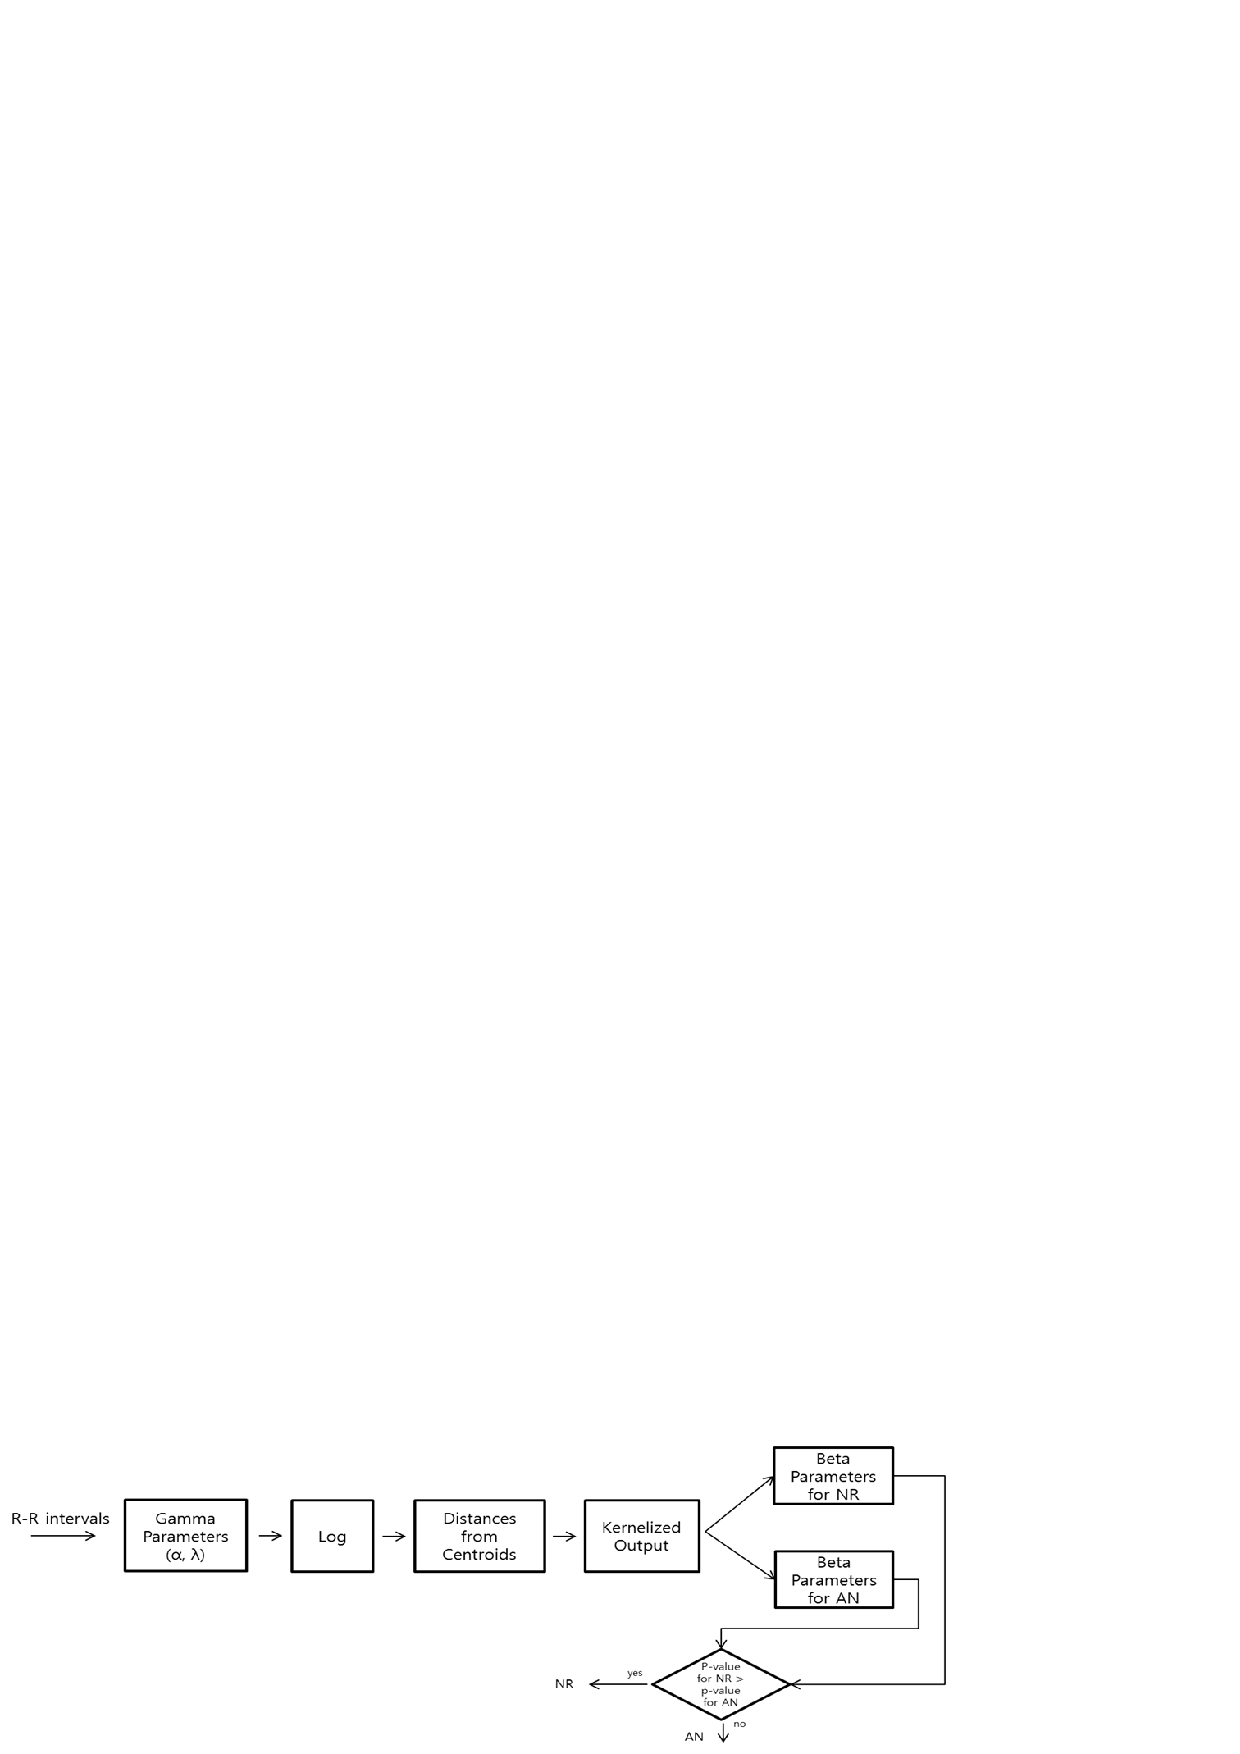
\includegraphics[width=17.4cm]{Fig_1.pdf}
\caption{The automatic classification system of heart condition using class probability output networks.}
\label{fig_system}
\end{figure*}

To solve this problem, the R-R intervals are analyzed  by the Gamma distribution parameters due to the fact that the random variable representing the interval between two random events follows a Gamma distribution. In this problem, the ECG signal can be described as the signal generated from the nonlinear and non-stationary system of heart activity. From this point of view, the Gamma parameters representing the distribution of R-R intervals in
a window of finite size are collected at every sampling time (for example, 10 seconds) and classified into the NR and AN features in the parameter space of Gamma distribution. Then, for these features, the classification of heart condition is made by using the class probability output network (CPON) 
(Park and Kil, 2009; Rosas et al., 2010) in which the conditional probability of heart condition given the feature of Gamma parameters is computed. For the proposed approach, the efficiency of classifying heart condition has been demonstrated through the simulation for classifying ECG signal data selected from 
the MIT-BIH Arrhythmia Database (Mark and Moody, 1988). In this simulation, the efficiency of CPON classifier has been demonstrated through the simulation for classifying ECG signal data and compared with other widely used classifiers such as the k-nearest neighbor (KNN) and support vector machine (SVM) classifiers.


This paper is organized as follows: in Section 2, the flow of classifying the heart condition is described; Section 3 contains a detailed description of the proposed method of classifying heart condition using the Gamma distribution of R-R intervals and also using the CPON classifier; in Section 4, the simulation for classifying heart condition using the proposed method has been demonstrated and compared with other classification methods; and finally, in Section 5, the conclusion of our work is presented.


\section{Automatic classification of heart conditions based on the HRV analysis}


In this problem of classifying the heart condition, the R-R intervals detected from the ECG signal data are collected over a window of finite size to obtain the statistically meaningful information of data distribution and make a decision for the heart condition. These procedure are assumed be done at every sampling time; that is, the classification of heart condition is done at every sampling time. In this classification of heart condition, the decision of NR heart condition is made when there are no abnormal ECG beats such as the VT, VB, and VF beats. Otherwise, the decision is made as the AN heart condition. The schematic diagram of the whole structure is illustrated in Figure~\ref{fig_system}. Here, the automatic classification of heart 
condition is constructed as follows: 1) the R-R intervals detected from the ECG signal data are collected within a window of fixed size (for example, 30 seconds) at every sampling time (for example, 10 seconds), 2) the parameters of Gamma distribution are obtained from these R-R intervals, 3) the log-scaled Gamma parameters are analyzed by calculating the distances between the estimated Gamma parameters and the previously learned centroids of Gamma parameters for the NR and AN classes of heart condition, 4) the kernelized output for the calculated distances is forwarded to the input of the CPON, 5) the p-values for testing the hypotheses of NR and AN classes are calculated using the Beta cumulative distribution functions (CDFs), 6) and then, the final decision is made by comparing the p-values for the NR and AN classes.

This method provides an accurate estimation of conditional class probabilities since in this training of classifiers, the Beta distribution parameters as well as the kernel parameters are adjusted in such a way that the output distributions of classifiers become closer to the ideal Beta distributions. Furthermore, the suggested CPON method is able to provide the degree of uncertainty for the final decision of classification (Rosas et al., 2010) by estimating the confidence intervals for the conditional class probabilities. 


\section{Features for HRV analysis}

 In HRV analysis, the time domain features are usually used for classifying heart condition. And the frequency domain features are also used for diagnosis of the heart diseases more precise (Metelka, 2014). There are statistical methods such as SDNN, SDANN, RMSSD, and geometric methods such as HRV triangular index. These features are calculated from N-N or R-R intervals in the short-term(5 min) or long-term(18-24 h). 1) SDNN is standard deviation of the all detected R-R intervals in the long-term. 

\begin{equation}
SDNN = {1\over{n-1}}\sqrt{\sum_{i=1}^{n}(RR_i - \overline{RR})^2},
\end{equation} 
 where n represents the total number of all detected R-R intervals, $RR_i$ and $\overline{RR}$ represent the $i$th detected R-R interval and the mean of all R-R intervals.
 2) SDANN is standard deviation of the averages of five-minute segments of all detected R-R intervals. If R-R intervals is detected for 24h, there are 288 segments.
\begin{equation}
SDANN = {1\over{S-1}}\sqrt{\sum_{i=1}^{S}(sRR_i-\overline{sRR})^2 },
\end{equation} where S represents the total number of the segments, $sRR_i$ and $\overline{sRR}$ represent the average of R-R intervals of $i$th segment and the mean of the averages of all segments. 3) RMSSD is the root mean square(RMS) of the differences between adjacency R-R intervals in the short-term. 
\begin{equation}
RMSSD = {1\over{n-1}}\sqrt{\sum_{i=1}^{n-1}(RR_i - RR_{i+1})^2}
\end{equation}
4) HRV triangular index, called geometric method, uses the histogram of the distribution of all detected R-R intervals in the long-term. After find the height of the histogram, the maximum number of the histogram. It is calculated from the total number of all detected R-R intervals divided by the height of the histogram. 

\
In the proposed method of classifying heart condition, the R-R intervals are analyzed by the Gamma distribution parameters ($\alpha$, $\lambda$) in which $\alpha$ and $\lambda$ determine the shape and scale of Gamma distributions, respectively. This analysis is possible due to the fact that the distribution of interarrival times (or intervals between two random events) can be described by the proper parameter values of Gamma distribution. In the case of interarrival times of independent events, this distribution becomes an exponential distribution; that is, the value of shape parameter α is equal to 1. From this point of view, the Gamma parameters for the distribution of R-R intervals are determined by the maximum likelihood estimation (MLE) method. For this purpose, the R-R intervals are extracted from the finite size window containing ECG waves. Then, the Gamma distribution parameters are determined in such a way of maximizing the likelihood function. First, the likelihood function $L(\alpha, \lambda)$ for $n$ observations of R-R intervals $(x_1, x_2, \cdots, x_n)$ is determined by
\begin{equation}
L(\alpha, \lambda) = \prod_{i=1}^n f(x_i| \alpha, \lambda),
\end{equation}        
where $f(x_i| \alpha, \lambda)$ represents the probability density function (PDF) of Gamma random variable defined by
\[
 f(x_i | \alpha, \lambda) = {1\over \Gamma (\alpha)}\lambda e^{-\lambda x_i}(\lambda x_i)^{\alpha -1} \; \; \mbox{and}\]
\[
\Gamma(\alpha) = \int_{0}^{\infty}\lambda e^{-\lambda x_i}(\lambda x_i)^{\alpha -1}dx_i.
\]
Then, the log-likelihood function is determined by
\begin{equation}
\log L(\alpha, \lambda) = (\alpha -1)\sum_{i=1}^n\log x_i - \sum_{i=1}^n{x_i\over \lambda} -
   n\log{{\lambda^{\alpha}}\over{\Gamma(\alpha)}}.
\end{equation}
From the above log-likelihood function, the maximum likelihood estimate of the parameter $\lambda$ is determined by
\begin{equation}
\hat{\lambda}={{\hat{\alpha} n}\over{\sum_{i=1}^n x_i}}. \label{lambda}
\end{equation}
Then, by substituting the estimate $\hat{\lambda}$  to the log-likelihood function $\log L(\alpha, \lambda)$ and taking the derivative of  
$\log L(\alpha, \lambda)$ with respect to $\alpha$, the maximum likelihood estimate $\hat{\alpha}$ can be found at the point where 
this derivative is equal to zero. As a result, the maximum likelihood estimate  $\hat{\alpha}$  is determined by
\begin{equation}
\hat{\alpha}\approx{{3-s+\sqrt{(s+3)^2+24s}}\over{12s}}, \label{alpha}
\end{equation}
where $s$ is given by
\[
s = \log({1\over n}\sum_{i=1}^nx_i) - {1\over n}\sum_{i=1}^n\log x_i.
\]
As an example of the estimation of Gamma parameters for the R-R intervals of ECG signal data, the Gamma parameters for a window of 30 seconds 
extracted from the MIT-BIH data sets were estimated using equations (3) and (4), and illustrated in Figure~\ref{fig_features_gamma}. 
This example demonstrated that 1) the NR and AN classes were well separated by Gamma parameters and 
2) there was more chance of occurring abnormal ECG patterns when the values of Gamma parameters ($\alpha$, $\lambda$) became smaller;
in this case, the dynamics of heart activity was changed and the variation of R-R intervals became larger compared with the normal ECG waves.

\
For comparision with the Gamma parameters and the statistical features, SDNN and RMSSD were calculated at the same windows and illustrated in Figure~\ref{fig_features_sdnn}, Figure~\ref{fig_features_rmssd} and Figure~\ref{fig_features_gamma_rmssd}.
\vspace{1em}

- Figure of (log alpha, log lambda, RMSSD)
\begin{figure}[!t]
\centering
\includegraphics[width=8.4cm]{Fig_gamma_params.pdf}
\caption{The NR and AN features in the log-scaled space of Gamma parameters.}
\label{fig_features_gamma}
\end{figure}
- Figure of SDNN
\begin{figure}[!t]
\centering
\includegraphics[width=8.4cm]{Fig_hist_SDNN.pdf}
\caption{The histograms of SDNN values of The NR and AN}
\label{fig_features_sdnn}
\end{figure}

- Figure of RMSSD
\begin{figure}[!t]
\centering
\includegraphics[width=8.4cm]{Fig_hist_RMSSD.pdf}
\caption{The histograms of RMSSD values of The NR and AN}
\label{fig_features_rmssd}
\end{figure}
- Figure of SDNN vs RMSSD
\begin{figure}[!t]
\centering
\includegraphics[width=8.4cm]{Fig_gamma_RMSSD.pdf}
\caption{The NR and AN features in the log-scaled Gamma parameters and The RMSSD values }
\label{fig_features_gamma_rmssd}
\end{figure}


\section{Classification algorithm for heart conditions}

After the estimation of Gamma parameters, they are log-scaled to cope with the range of heart dynamics. Then, in the space of log-scaled Gamma parameters, the centroids representing the distributions of normal and abnormal classes are searched using the clustering algorithm such as the LBG algorithm 
(Linde et al., 1980) which is an expectation and maximization (EM) method of determining centroids. In this clustering algorithm, the NR and AN classes are respectively represented by 22 and 11 clusters according to the sampling ratio of around 140 to 1. Then, for each centroid, a Gaussian kernel function is allocated. Here, the Gaussian kernel function for the given input pattern ${\bf x} = [x_1, x_2]^t$  is given by 
\begin{equation}
\phi_j({\bf x}) = e^{-cd_j^2({\bf x})}, \; \; \; d_j^2({\bf x}) = \sum_{i=1}^2{{(x_i - u_{ij})^2}\over{2\sigma_{ij}^2}}, \label{kernel}
\end{equation}
where $c$ is a constant term related with the dispersion of Gaussian function,
$\mu_{ij}$ and $\sigma_{ij}$ represent the mean and standard deviation of the $i$th coordinate of the $j$th centroid, respectively.
Here, the value of $c$ is determined in such a way of finding the proper distribution of classification output (in our case, the Beta distribution).
By the linear combination of Gaussian kernel functions, the decision function of classifying heart conditions is given as follows:
\begin{equation}
y({\bf x})=\sum_{j=1}^m w_i\phi_j({\bf x}), \label{y(x)}.
\label{decision}
\end{equation}
Then, the next step is to determine the weights of (6) in such a way of discriminating the normal and abnormal heart conditions. For this purpose, the linear discriminant analysis (LDA) (Duda et al., 2001) can be applied. First, for $n$ input patterns in the space of log-scaled Gamma parameters
 \[
{\bf x}_i = [x_{1i}, x_{2i}]^t, \; \; \; i= 1, \cdots, n,
\]
the kernelized output patterns are defined by
\[
\tilde{\bf x}_i = [\phi_1({\bf x}_i), \cdots, \phi_m({\bf x}_i)]^t \; \; \; i= 1, \cdots, n.
\]
Here, we assume that the number of patterns $n$ given by
\[
n = n_{nr} + n_{an},
\]
where $n_{nr}$ and $n_{an}$ represent the number of normal and abnormal classes, respectively.

From these kernelized output patterns, the mean vectors of normal and abnormal classes are defined by
\[
{\bf m}_{nr} = {1\over n_{nr}}\sum_{\tilde{\bf x}_i\in D_{nr}} \tilde{\bf x}_i \; \; \; \mbox{and}
\]
\[
{\bf m}_{an} = {1\over n_{an}}\sum_{\tilde{\bf x}_i\in D_{an}} \tilde{\bf x}_i, 
\]
where ${\bf m}_{nr}$ and ${\bf m}_{an}$ represent the mean vectors for the normal and abnormal classes, respectively, and 
$D_{nr}$ and $D_{an}$ represent the collection of kernelized output patterns for the normal and abnormal classes, respectively.

Then, the scatter matrices for the normal and abnormal classes are defined by
\[
S_{nr} = \sum_{\tilde{\bf x}_i\in D_{nr}}(\tilde{\bf x}-{\bf m}_{nr})(\tilde{\bf x}-{\bf m}_{nr})^t \; \; \; \mbox{and}
\]
\[
S_{an} = \sum_{\tilde{\bf x}_i\in D_{an}}(\tilde{\bf x}-{\bf m}_{an})(\tilde{\bf x}-{\bf m}_{an})^t,
\]
where $S_{nr}$ and $S_{an}$ represent the scatter matrices for the normal and abnormal classes, respectively.

By summing the scatter matrices for the normal and abnormal classes, the following within the scatter matrix $S_{w}$ is defined:
\[
S_{w} = S_{nr} + S_{an}.
\]
For the difference of mean vectors between the normal and abnormal classes, the between the scatter matrix $S_b$ is also defined as follows:
\[
S_{b} = ({\bf m}_{nr} - {\bf m}_{an})({\bf m}_{nr} - {\bf m}_{an})^t.
\]

Then, the weight vector associated with kernels
\begin{equation}
{\bf w} = [w_1, w_2, \cdots, w_m]^t,
\end{equation}
is determined in such a way of minimizing the following LDA criterion:
\begin{equation}
J({\bf w})={{{\bf w}^tS_b{\bf w}}\over{{\bf w}^tS_w{\bf w}}}.
\end{equation}
This implies that the weight vector is determined by maximizing the difference between two mean vectors of normal and abnormal classes while
minimizing the variance of each class. As a result, the mean vector is determined by
\begin{equation}
{\bf w} = S_w^{-1}({\bf m}_{nr} - {\bf m}_{an}). \label{w}
\end{equation}

After the construction of decision function of (6), the output distribution of decision function $y$ is identified by the Beta distribution for the probabilistic representation of classifier output. In fact, the distribution of the classifier output can be approximated by the Beta distribution under the assumption that the classifier output has an unimodal distribution; that is, one output value corresponding to the greatest frequency exists, and the range of output values is finite. Under these assumptions, the PDF $f_Y$ of a Beta random variable $Y$ whose values lies between 0 and 1 is determined by
\begin{equation}
f_Y(y|a, b) = \frac{1}{B(a, b)}y^{a-1}(1-y)^{b-1},
\end{equation}
where $a$ and $b$ represent positive constants for the Beta density function, and $B(a, b)$ represents the Beta function defined by
\[
B(a, b) = \int^1_0 y^{a-1}(1-y)^{b-1}dy.
\]
Here, we assume that the values of the classifier's output are normalized between 0 and 1.  

Then, the CDF of Beta random variable $Y$ is described by
\begin{equation}
F_Y(y|a, b) = \frac 1 {B(a, b)}\int^y_0 x^{a-1}(1-x)^{b-1}dx. \label{F_Y}
\end{equation}
One of the advantages of the beta distribution is that the Beta distribution parameters can be easily guessed from 
the mean E[Y] and variance Var(Y) as follows:
\begin{equation}
a =  E[Y]\left( {{E[Y](1-E[Y])}\over Var(Y)}-1
\right) \; \; \mbox{and}\label{p_alpha}
\end{equation}
\begin{equation}
b = (1-E[Y])\left( {{E[Y](1-E[Y])}\over Var(Y)}-1
\right).\label{p_beta}
\end{equation}
Although this moment matching (MM) method is simple, these estimators usually don't provide accurate estimations especially for smaller number of data. 
To cope with this problem, the Beta parameters can be determined in such a way of maximizing the log-likelihood function of Beta parameters for 
$n$ output values of $y_i, i=1, \cdots, n$ given by
\begin{eqnarray}
L(a, b) = -n\log B(a, b) +  \; \; \; \; \; \; \; \; \; \; \; \; & & \nonumber \\
\; \; \; (a-1)\sum_{i=1}^n\log (y_i) + (b-1)\sum_{i=1}^n\log(1-y_i). & & \label{L_beta}
\end{eqnarray}
To solve this MLE method, the Beta parameters should be searched using the extremum points of the log-likelihood function; they are
\begin{equation}
{\partial\over {\partial a}}\log L(a, b)|_{a=\hat a, b=\hat b} = 0 \; \;\;  \mbox{and}
\end{equation}
\begin{equation}
{\partial\over {\partial b}}\log L(a, b)|_{a=\hat a, b=\hat b} = 0
\end{equation}
Then, from the above equations, the Beta parameters can be estimated using the iteratively searching method of finding solutions such as 
the Newton-Raphson method (AbouRizk et al., 1994).
As an example of the estimation of Beta parameters, the output distributions of (\ref{y(x)}) for the NR and AN classes are identified by Beta parameters and illustrated in Figure~\ref{fig_CPON}.

\begin{figure}[!t]
\centering
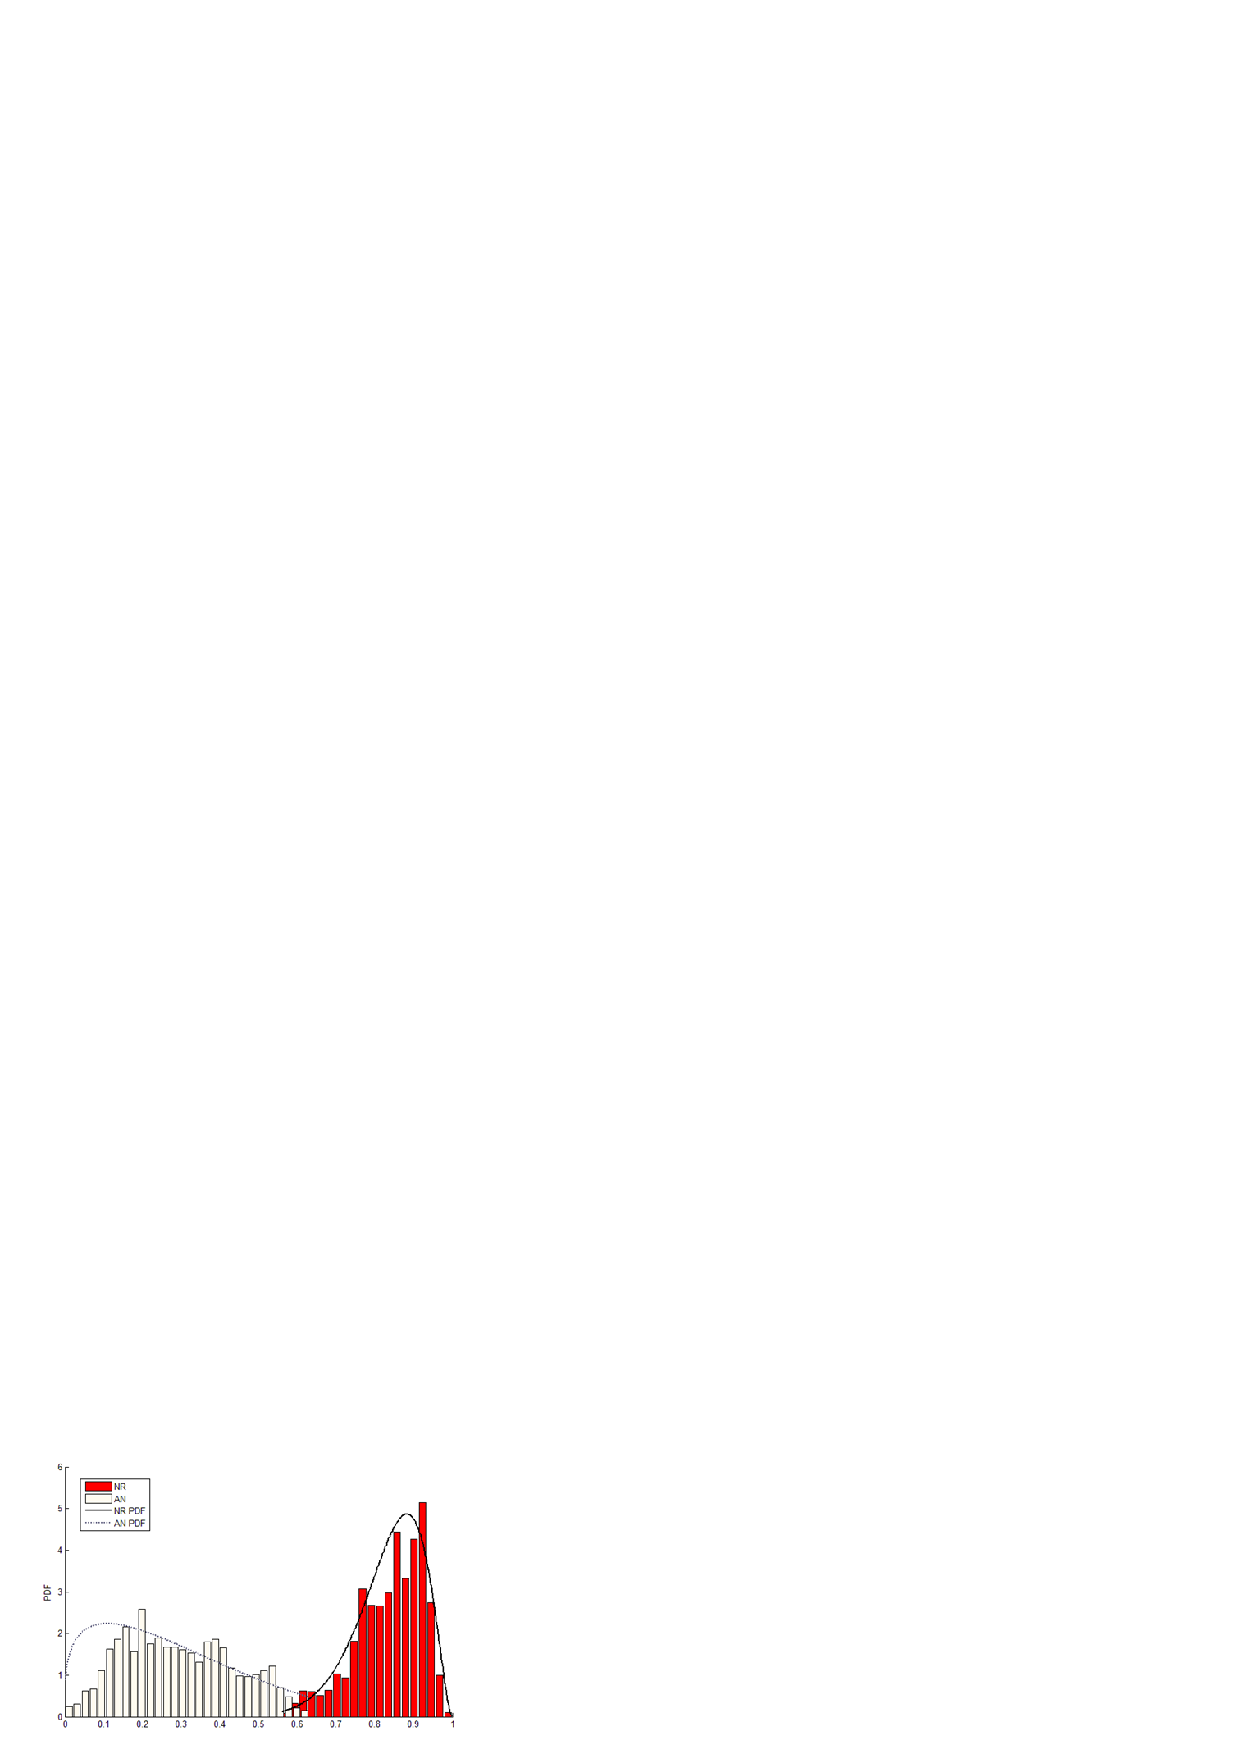
\includegraphics[width=8.4cm]{Fig_3.pdf}
\caption{The Beta distributions for the NR and AN classes: bars represent frequencies, and the solid and dotted lines represent 
the estimated Beta PDFs for the normal and abnormal classes, respectively.}
\label{fig_CPON}
\end{figure}

After the estimation of Beta parameters, each distribution of NR or AN class represents the hypothesis of the given condition; that is,
the Beta CDF value of (\ref{F_Y}) can be considered as the $p$-value for testing the NR or AN class; that is,
\begin{equation}
\mbox{$p$-value$^{nr}$} = \Pr\{Y^{nr}\le y\}
= F_{Y^{nr}}(y) \; \mbox{or}
\end{equation}
\begin{equation}
\mbox{$p$-value$^{an}$} = \Pr\{Y^{an}\ge y\}
= 1 - F_{Y^{an}}(y),
\end{equation}
where $Y^{nr}$ and $Y^{an}$ respectively represent the random variables for the normal and abnormal classes, and
$p$-value$^{nr}$ and $p$-value$^{an}$ respectively represent the $p$-values for testing the NR and AN classes.

Then, the probability of the normal or abnormal classes of heart condition for the given R-R intervals
can be evaluated as the $p$-value ratio of  testing the NR and AN classes; that is,
\begin{equation}
\mbox{$\Pr^{nr}$} = {{\mbox{$p$-value$^{nr}$}}\over{\mbox{$p$-value$^{nr}$}+\mbox{$p$-value$^{an}$}}}, \label{p_ratio}
\end{equation}
where $\mbox{$\Pr^{nr}$}$ represent the probability of normal heart condition while $\mbox{$\Pr^{an}$}=1 - \mbox{$\Pr^{nr}$}$ 
represent the probability of abnormal heart condition.
From this probability, the final decision of normal and abnormal classes can be made as follows:
\begin{equation}
\mbox{heart condition} = \left\{ \begin{array}{ll}
                                      \mbox{normal}     & \mbox{if $\Pr^{nr} \ge 0.5$}\\
                                      \mbox{abnormal} & \mbox{otherwise.} \end{array} \right.
\end{equation}

In summary, the learning algorithm of classifying heart condition is described as follows:
\begin{description}
\item[Step 1.] For an input pattern of R-R intervals within a finite window, determine the values of
  Gamma parameters $(\alpha, \lambda)$ using the equations (\ref{lambda}) and (\ref{alpha}). Then, collect the set of Gamma parameters for
  the NR and AN heart classes from the input patterns.
\item[Step 2.] Then, in the space of ($\log \alpha$, $\log \lambda$), the centroids representing the local distribution of
  patterns are determined by the clustering algorithm such as the LBG algorithm (Linde et al., 1980).
\item[Step 3.] At each centroid, the kernel function of (\ref{kernel}) is located and the kernel width is determined
  according to the standard deviation of the centroid.
\item[Step 4.] Then, for the decision function of (\ref{y(x)}), the associated weight vector is determined by the LDA method 
  (Duda et al., 2001); that is, the weight vector is determined by the equation (\ref{w}).
\item[Step 5.] From the output distribution of decision function, the values of Beta parameters ($a$, $b$) can be determined by the moment
  matching (MM) method; that is, ($a$, $b$) are determined by the equations (\ref{p_alpha}) and (\ref{p_beta}), or for more accurate estimation of
Beta parameters, the MLE method (AbouRizk et al., 1994) maximizing the log-likelihood function of (\ref{L_beta}) can be applied.
\end{description}

Then, after the construction of CPON-based classifier, the probability of the NR and AN classes for the given R-R intervals
can be determined by the equation (\ref{p_ratio}).
However, in general, these probability estimates of Gamma and Beta distribution parameters may not be optimal
due to not enough number of data.  If these estimates are accurate, the distribution of the cumulative
distribution function of data; that is, $F_Y(Y_i), \; i=1, \cdots,
n$ becomes uniformly distributed by the following reason:
\begin{itemize}
\item Let us consider random variables 

$U_i=F_Y(Y_i), \; i=1, \cdots, n$; then,
\item each $U_i$ has uniform distribution because its probability
density function is given by
\[
f_U(u)={{f_Y(y)}\over{|{{dF_Y}/{dy}}|}}={{f_Y(y)}\over{|f_Y(y)|}}=1,
\]
where $u=F_Y(y)$.
\end{itemize}
From this point of view, we need to check the uniformity of
$F_Y(Y_i)$, $i=1, \cdots, n$ using the hypothesis test such as the
Kolmogorov-Smirnov (K-S) test (Rohatgi and Saleh, 2001) which is performed for the
empirical cumulative distribution function (ECDF). The procedure of
the K-S test is given as follows:
\begin{itemize}
\item Let ${\cal S}_Y=\{Y_i | i=1, \cdots, n\}$ be a sample from the CDF
$F_Y$, and let $F_n^*$ be the corresponding ECDF. Then, the K-S
statistic $D_n$ is defined by
\begin{equation}
D_n = \sup_{y\in {\cal S}_Y}|F_n^*(y) - F_Y(y)|. \label{D_n}
\end{equation}
In the case of uniform distribution, $F_Y(y) = y$.
\item The K-S statistic $D_n$ can be used to test the following
hypotheses:
\[
H_0: F_n^*(y)=F_Y(y) \; \; \mbox{versus} \; \; H_1: F_n^*(y)\neq
F_Y(y).
\]
Let the value of $D_n$ be $d_n$.  Then, to test these hypotheses, we
can calculate the $p$-value from the K-S distribution:
\begin{equation}
p \textrm{-value} = \Pr\left\{ D_n \geq \frac{t}{\sqrt{n}}\right\} =
1-H(t), \label{p_val}
\end{equation}
where $t$ represents a variable defined by t = $\sqrt{n}d_n$ and
$H(t)$ represents the CDF of the K-S statistic determined by
\[
H(t) = 1- 2\sum_{i=1}^\infty (-1)^{i-1}e^{-2i^2t^2}. \label{H_t}
\]
\item Finally, the testing of the hypotheses at a significance level $\delta$ is to
\[
\mbox{accept $H_0$, if $p$-value $\ge$ $\delta$; reject $H_0$,
otherwise.}\]
\end{itemize}
If the data $F_n^*(Y_i)$, $i=1, \cdots, n$ pass the hypothesis test
of uniform distribution, it implies that the estimates of Gamma or Beta parameters are good enough to represent the distribution of the
classifier's output. For the proposed method, the K-S tests whether the estimated Gamma or Beta parameters were fitted to
the given data distribution, were performed. In these tests, the MIT-BIT data sets were used as the benchmark data sets. As a result, the 
$p$-values for K-S tests were obtained as listed in Table~\ref{T1}. As shown in these $p$-values, they were much greater than the usual value of the level of significance (= 0.05); that is, the estimation of Gamma and Beta parameters were well fitted to the given data distributions.

Some attractive features of the proposed method are as follows: 1) there is no need to make an assumption about class output distributions, 2) the proposed method can be used for an unbalanced data set because the ratio of the number of data for each class is not important, rather the number of data itself is important for the accurate estimation of Beta distribution parameters, and 3) the Beta distribution parameters as well as the kernel parameters can be adjusted for the accurate estimation of classifier output distribution and this estimation can be evaluated by the hypothesis test for data distribution such as the K-S test. As a result, the better estimation of posterior probabilities of class membership is possible and this contributes the improvement of the classification performances. 

\begin{table}
\caption{The $p$-values for testing the Gamma and Beta distribution parameters} \label{T1}
\begin{center}
\begin{tabular}{|c||c|c|}\hline\hline
                   & NR     & AN   \\ \hline\hline
Gamma       & 0.6083  & 0.5959 \\ \hline
Beta            & 0.3127  & 0.1733 \\ \hline
\end{tabular}
\end{center}
\end{table}

\section{Simulation for the classification of heart conditions}

To show the effectiveness of the proposed method, the ECG signal data from the MIT-BIH Arrhythmia Database were selected. The MIT-BIH Arrhythmia Database contains 48 half-hour ECG recordings from 47 subjects. For this simulation, 23 recordings were chosen from a set of a mixed population of inpatients ($60\%$) and outpatients ($40\%$) at Boston Beth Israel Hospital. The remaining 25 recordings were selected from the same set but clinically significant arrhythmias that would not be well represented in a random sample of small size. Annotations for the normal beats and abnormal beats including the VT, VB, and VF beats, and more beats were labeled by two independent cardiologists and it had approximately 109,000 beat labels. A window of 30 seconds for ECG signal data was selected and the R-R intervals in a window was used as an input pattern, and sequences of input patterns sampled at every 10 seconds were collected as the data set for the classification of NR and AN classes. As a result, a set of 3,198 NR and 1,565 AN patterns was used as the data set for the classification of  NR and AN classes. 

In the proposed method, the Gamma parameters were estimated using the equations (3) and (4). Then, in the space of log-scaled Gamma parameters, the LBG algorithm was applied so that 22 and 11 centroids were obtained for the NR and AN classes, respectively. At each position of centroid, the Gaussian kernel function was located as shown in the equation (5) with the value of $c=1/\pi$ and the weight vector of the decision function of (6) was determined by the LDA method as shown in the equation (9). Then, the Beta parameters were obtained in such a way of minimizing the log-likelihood function of (14). For the comparison of the proposed CPON classifier with other classifiers, the popular classification 
models such as the kNN and SVM classifiers were trained for the input data of log-scaled Gamma parameters and the output data of the labels of NR and AN classes. For these classifiers, Scikit-learn Python library (Pedregosa et al., 2011) was used for the training of the given data set. In the case of kNN classifier, the nearest neighbor; that is, $k = 1$ was used with the default setting of other parameters. For the SVM classifier, the support vectors were selected using the linear kernels. In this simulation, each classifier was evaluated by the 10-fold cross-validation method in which the the given data set was split into 10 parts evenly for the NR and AN patterns. Among 10 parts, one part was used as the test data, and the remaining 9 out of 10 parts were used as the training data. Then, the classification performances for the test data were obtained. This cross-validation process is repeated 10 times in which each of 10 parts was used exactly once as the test data. Then, the average values of classification performances for 10 subparts of data set were obtained as the simulation results.

For the classification performances, there are four standard performance measures: the accuracy, precision, recall, and $F_1$ measures. 
The accuracy measure represents one minus the ratio of the wrong assignments over the total number of assignments; that is,
\begin{equation}
Accuracy=1- {{|FP|+|FN|}\over{|TP|+|FP|+|TN|+|FN|}},
\end{equation}
where $TP$, $TN$, $FP$, and $FN$ represents the true positives, true negatives, false positives, and false negatives, respectively.
 
The precision measure $p$ represents the ratio of true positives over the total of positive assignments:
\begin{equation}
p= {|TP|\over{|TP|+|FP|}}.
\end{equation}

The recall measure $r$ is defined as the ratio of true positives over the total of correct assignments:
\begin{equation}
r= {|TP|\over{|TP|+|FN|}}.
\end{equation}

Finally, the $F_1$ measure, a trade-off between the precision and recall, is defined by
\begin{equation}
F_1= {2pr\over{p+r}}.	
\end{equation}

\iffalse
\begin{table}[!t]
\caption{Classification performances for the NR and AN classes using three classification methods when the positive class is NR} \label{T2}
\begin{center}
\begin{tabular}{|c|c|c|c|c|}\hline\hline
\multicolumn{2}{|c|}{}& kNN     & SVM   & CPON \\ \hline\hline
\multicolumn{2}{|c|}{Accuracy}         
& 0.9796  & 0.9689  & {\bf 0.9773} \\ \hline
\multirow{3}{*}{Positive NR} &  Precision 
& 0.9844  & 0.9790  & {\bf 0.9687} \\ \cline{2-5}
& Recall   
& {\bf 0.9853}  & 0.9583 & 0.9974 \\ \cline{2-5}
& $F_1$ Measure 
& 0.9848  & {\bf 0.9686} & 0.9829 \\ \hline
\multirow{3}{*}{Positive AN} &  Precision  
& 0.9700  & 0.9790  & {\bf 0.9949} \\ \cline{2-5}
& Recall   
& {\bf 0.9681}  & 0.9583 & 0.9397 \\ \cline{2-5}
& $F_1$ Measure 
& 0.9690  & {\bf 0.9686} & 0.9665 \\ \hline
\end{tabular}
\end{center}
\end{table}

\begin{table}[!t]
\caption{Classification performances for the NR and AN classes using three classification methods when the positive class is AN} \label{T3}
\begin{center}
\begin{tabular}{|c|c|c|c|}\hline\hline
                      & kNN     & SVM   & CPON \\ \hline\hline
Accuracy         & 0.9583  & 0.9689  & {\bf 0.9692} \\ \hline
Precision         & {\bf 0.9624}  & 0.9592  & 0.9479 \\ \hline
Recall             & 0.9538  & 0.9795 & {\bf 0.9930} \\ \hline
$F_1$ Measure & 0.9581  & 0.9692 & {\bf 0.9699} \\ \hline
\end{tabular}
\end{center}
\end{table}
\fi
%After performing the classification of the NR and AN classes using three types of classification methods, the performances of classification results were obtained as shown in Tables II and III. These simulation results showed that 1) three classifiers provided high accuracies (over 0.95) of classification performances and 2) the proposed CPON method provided higher precision for the normal heart condition and higher recall for the abnormal heart condition than other methods. These results imply that 1) the Gamma parameters are good features for the classification of NR and AN classes, and 2) the proposed CPON is favorable for detecting possibly abnormal heart condition due to higher recall (over 0.99) for the abnormal heart condition than other methods. Furthermore, the proposed CPON method is able to provide the probabilities of normal or abnormal heart condition for the given R-R intervals using the $p$-value ratio of (19).

\vspace{1em}

- Simulation results 1: (log $\alpha$, log $\lambda$), (SDNN), (RMSSD), (SDNN, RMSSD)

 (log $\alpha$, log $\lambda$), (SDNN), and (RMSSD) model was with two kernels (each classes) and kernel  parameter = 0.9 ,  (SDNN, RMSSD) model was with 22 kernels for the NR and 11 kernels for the AN. (log $\alpha$, log $\lambda$) out of all features was the best performances of all measurements.
\begin{table*}[!t]
\caption{Classification performances for the NR and AN classes of the CPONs trained by various features when the positive class is NR} \label{Table_sim1}
\begin{center}
\begin{tabular}{|c|c|c|c|c|c|}\hline\hline
\multicolumn{2}{|c|}{}& log $\alpha$, log $\lambda$     & SDNN   & RMSSD & SDNN, RMSSD \\ \hline\hline
\multicolumn{2}{|c|}{Accuracy}         
& {\bf 0.9796}  & 0.9225  & 0.9343 & 0.9301\\ \hline
\multirow{3}{*}{Positive NR} &  Precision 
& {\bf 0.9734}  & 0.9112  & 0.9331 &0.9024 \\ \cline{2-6}
& Recall   
& {\bf 0.9961}  & 0.9717 & 0.9679 &0.9928 \\ \cline{2-6}
& $F_1$ Measure 
& {\bf 0.9847}  & 0.9405 & 0.9502 & 0.9455\\ \hline
\multirow{3}{*}{Positive AN} &  Precision  
& {\bf 0.9923}  & 0.9457  & 0.9367 &0.9866\\ \cline{2-6}
& Recall   
& {\bf 0.9481}  & 0.8390 & 0.8726 &0.8319\\ \cline{2-6}
& $F_1$ Measure 
& {\bf 0.9697}  &  0.8892 & 0.9035 &0.9027\\ \hline
\end{tabular}
\end{center}
\end{table*}

\begin{table*}[!t]
\caption{Classification performances for the NR and AN classes of the CPONs trained by various features when the positive class is NR} \label{Table_sim2}
\begin{center}
\begin{tabular}{|c|c|c|c|c|}\hline\hline
\multicolumn{2}{|c|}{}& log $\alpha$, log $\lambda$     & SDNN   & RMSSD  \\ \hline\hline
\multicolumn{2}{|c|}{Accuracy}         
& 0.9824  & 0.9798  & {\bf 0.9855} \\ \hline
\multirow{3}{*}{Positive NR} &  Precision 
& 0.9778  & 0.0.9744  & {\bf 0.9894}  \\ \cline{2-5}
& Recall   
& {\bf 0.9959}  & 0.9955 & 0.9891 \\ \cline{2-5}
& $F_1$ Measure 
& 0.9867  & 0.9848 & {\bf 0.9892} \\ \hline
\multirow{3}{*}{Positive AN} &  Precision  
& {\bf 0.9917}  & 0.9911  & 0.9776 \\ \cline{2-5}
& Recall   
& 0.9563  & 0.9498 & {\bf 0.9783} \\ \cline{2-5}
& $F_1$ Measure 
& 0.9737  &  0.9700 & {\bf 0.9779} \\ \hline
\end{tabular}
\end{center}
\end{table*}
- Simulation results 2: (log $\alpha$, log $\lambda$, SDNN), (log $\alpha$, log $\lambda$, RMSSD), (log $\alpha$, log $\lambda$, Skewness)
 models were trained by kernel parameter = 0.4 with 22 kernels for the NR and 11 kernels for the AN.
 




- Simulation results 3: for simulation results 2, compare the performances of the KNN, SVM, and CPON




\section{Conclusion}

For the classification of heart condition, the R-R intervals of ECG signal data are analyzed by the parameters of Gamma distribution in the proposed approach. 
Then, these parameter values as the representatives of ECG signal data are classified into the normal (NR) heart condition or the abnormal (AN) heart condition
in which there exists abnormal ECG beats such as the ventricular tachycardia (VT), ventricular bigeminy (VB), and ventricular fibrillation (VF) beats.
The classification of the NR or AN heart condition is performed by estimating
the condition class probabilities using class probability output networks (CPONs). As a result, the heart condition is identified in a consistent and reliable manner. Through the simulation for classifying heart condition using the MIT-BIH data sets, it has been demonstrated that the Gamma parameters are effective features for classifying heart condition and the classification using CPONs is favorable for detecting possibly abnormal heart condition due to higher recall for the abnormal heart condition than other methods. Furthermore, the proposed method is able to provide the probabilities of  normal or abnormal heart condition for the given heart data of R-R intervals or 
beat-to-beat intervals by calculating the $p$-values for testing the normal and abnormal classes.
The proposed method can be easily applied to various handheld or wearing devices including smart watches with heart rate sensors
due to the fact that this method only requires a sequence of beat-to-beat intervals as the input pattern.

%\section*{Acknowledgments}
%This research was supported in part by the Research Program of  the College of Information and Communication Engineering, Sungkyunkwan University.

\section*{References}

\begin{enumerate}
\item Y. Hu, S. Palreddy, and W. Tompkins, 1997. A patient adaptable ECG beat classifier using a mixture of experts approach.
     IEEE Transactions on Biomedical Engineering 44, 891-900.
\item K. Minami, H. Nakajima, and T. Toyoshima, 1999. Real-time discrimination of ventricular tachyarrhythmia with Fourier-transform neural network.
     IEEE Transactions on Biomedical Engineering 46, 179-185.
\item N. Thakor, Y. Zhu, and K. Pan, 1990. Ventricular tachycardia and fibrillation detection by a sequential hypothesis testing algorithm.
     IEEE Transactions on Biomedical Engineering 37, 837-843.
\item N. Thakor, A. Natarajan, and G. Tomaselli, 1994. Multiway sequential hypothesis testing for tachyarrhymia discrimination.
     IEEE Transactions on Biomedical Engineering 41, 480-487.
\item J. Willems and E. Lesaffre, 1987. Comparison of multigroup logistic and linear discriminant ECG and VCG classification.
     Journal of Electrocardiology 20, 83-92.
\item D. Gao, M. Madden, D. Chambers, and G. Lyons, 2005. Bayesian ANN classifier for ECG arrhythmia diagnostic system: a comparison study.
     In: Internat. Joint Conf. on Neural Networks, pp. 2383-2388.
\item R. Silipo and C. Marchesi, 1998. Artificial neural networks for automatic ECG analysis.
     IEEE Transactions on Signal Processing 46, 1417-1425.
\item A. Coast, R. Stern, G. Cano, and S. Briller, 1990. An approach to cardiac arrhythmia analysis using hidden Markov models.
     IEEE Transactions on Biomedical Engineering 37, 826-835.
\item S. Osowski and T. Linh, 2001. ECG beat recognition using fuzzy hybrid neural network.
     IEEE Transactions on Biomedical Engineering 48, 1265-1271.
\item Y. Wang, Y. Zhu, N. Thakor, and Y. Xu, 2001. A short-time multifractal approach for arrhythmia detection based on fuzzy neural network.
     IEEE Transactions on Biomedical Engineering 48, 989-995.
\item W. Jiang and S. Kong, 2007. Block-based neural networks for personalized ECG classification.
     IEEE Transactions on Neural Networks 18, 1750-1761
\item W. Park and R. Kil, 2009. Pattern classification with class probability output network.
     IEEE Transactions on Neural Networks 20, 1659-1637.
\item H. Rosas, R. Kil, and S. Han, 2010. Automatic media data rating based on class probability output networks.
     IEEE Transactions on Consumer Electronics 56, 2296-2302.
\item R. Mark and G. Moody, 1988. MIT-BIH Arrhythmia Database Directory, MIT, Cambridge, MA.
\item Y. Linde, A. Buzo, and R. Gray,1980. An algorithm for vector quantizer design.
     IEEE Transactions on Communication 28, 84-95.
\item R. Duda, P. Hart, and D. Stork, 2001. Pattern Classification, John Wiley \& Sons, Inc.
\item M. AbouRizk, W. Halpin, and R. Wilson, 1994. Fitting beta distributions based on sampled data.
     Journal of Construction and Management 120, 288-305.
\item V. Rohatgi and A. Saleh, 2001. Nonparametric statistical inference. In:
     An Introduction to Probability and Statistics, 2nd ed., Wiley-Interscience, New York.
\item F. Pedregosa et al., 2011. Scikit-learn: machine learning in Python.
     Journal of Machine Learning Research 12, 2825-2830.
\item R. Metelka, 2014. Heart rate variability - current diagnosis of the cardiac autonomic neuropathy. Biomed Pap Med Fac Univ Palacky Olomouc Czech Repub 158 (3), 327-338.
\end{enumerate}

\bibliographystyle{model2-names}
\bibliography{refs}

\end{document}

%%
